\documentclass[withoutpreface]{cumcmthesis}

\title{B题 问题一：数据整理与快充策略寿命差异初步分析}
\tihao{B}
\baominghao{123456}
\schoolname{XX大学}
\membera{成员A}
\memberb{成员B}
\memberc{成员C}
\supervisor{指导教师}
\yearinput{2026}
\monthinput{08}
\dayinput{01}

\usepackage{booktabs}
\usepackage{graphicx}
\usepackage{float}

\begin{document}

\maketitle

\begin{abstract}
本文基于MIT--Stanford锂离子电池循环老化数据集，对138块A123 18650型磷酸铁锂电池的快充策略与循环寿命进行了系统整理和初步分析。
首先从原始实验数据中提取了各电池的充电策略、SOH衰减曲线、循环寿命和充电时间等关键信息，获得70种不同的快充策略。
随后对寿命分布进行了统计分析，发现循环寿命从148次到1935次不等，呈宽分布特征。
通过选取典型长寿命策略（4.8C(80\%)-4.8C，平均寿命1564次）和短寿命策略（2C(10\%)-6C，寿命仅148次），
从充电倍率、SOC切换节点和充电时间三个维度对寿命差异进行了解释。
初步分析表明：第二阶段充电倍率C2和SOC切换节点Q1是影响循环寿命的关键因素，而低SOC区间的第一阶段倍率C1对寿命的影响相对有限。
\keywords{锂离子电池\quad 快充策略\quad 循环寿命\quad SOH衰减\quad SOC区间}
\end{abstract}

\section{问题重述}

\subsection{研究背景}
随着新能源汽车和储能系统的快速发展，锂离子电池的快充性能直接影响用户体验和系统运行效率。
快速充电能够显著缩短补能时间，但较高的充电电流也可能加速电池老化，导致容量衰减加快和循环寿命缩短。
数据集中的电池采用两段式快充策略：第一阶段以倍率$C_1$从0\% SOC充电至$Q_1$，第二阶段以倍率$C_2$从$Q_1$充电至80\% SOC，随后以1C恒流-恒压模式充满。

\subsection{问题要求}
问题一要求对原始循环实验数据进行整理，提取各电池的充电策略、充电时间、SOH变化及循环寿命等关键信息，
给出典型长寿命和短寿命策略，并从充电电流倍率大小、SOC区间和充电时间角度进行初步解释。

\section{数据整理方法}

\subsection{数据集概况}
数据来源于MIT--Stanford公开锂离子电池循环老化数据集\cite{severson2019}，包含三个批次共138块A123 18650型磷酸铁锂电池的循环老化实验数据。
各电池放电策略相同，仅充电策略存在差异，天然构成控制变量实验条件。

\subsection{数据提取流程}
针对每块电池，从MATLAB格式原始文件（data\_1.mat, data\_2.mat, data\_3.mat）中提取以下关键信息：

\begin{enumerate}
    \item \textbf{充电策略参数}：从可读策略字符串（如``3.6C(80\%)-3.6C''）中通过正则匹配提取第一阶段倍率$C_1$、SOC切换节点$Q_1$和第二阶段倍率$C_2$；
    \item \textbf{循环寿命}：从cycle\_life字段直接获取SOH衰减至80\%时的循环次数；
    \item \textbf{SOH衰减曲线}：利用每次循环的放电容量$Q_{\text{Discharge}}$计算SOH：
    \begin{equation}
        \text{SOH}(n) = \frac{Q_{\text{Discharge}}(n)}{Q_{\text{initial}}}
    \end{equation}
    其中$Q_{\text{initial}}$取前5次循环的最大放电容量；
    \item \textbf{充电时间}：从summary数据中提取每次循环的充电时间，计算平均充电时间。
\end{enumerate}

经清洗，剔除2块无循环寿命数据的电池和3块策略参数无法解析的电池，最终获得133块有效电池数据，覆盖70种不同的充电策略。

\section{结果与分析}

\subsection{循环寿命总体分布}

133块电池的循环寿命统计特征如表\ref{tab:life_stats}所示。

\begin{table}[H]
\centering
\caption{循环寿命统计特征}
\label{tab:life_stats}
\begin{tabular}{lc}
\toprule
统计量 & 数值（次循环） \\
\midrule
样本数 & 133 \\
均值 & 791.5 \\
中位数 & 787.0 \\
标准差 & 322.3 \\
最小值 & 148.0 \\
25\%分位数 & 499.8 \\
75\%分位数 & 987.3 \\
最大值 & 1935.0 \\
\bottomrule
\end{tabular}
\end{table}

寿命分布呈现宽分布特征（标准差322次），最长的电池寿命（1935次）是最短的（148次）约13倍，
说明不同充电策略对电池寿命的影响极为显著。

\subsection{典型策略对比}

将所有策略按中位循环寿命排序，选取排名前3的长寿命策略和排名后3的短寿命策略进行详细对比，
结果如表\ref{tab:typical}和图\ref{fig:soh}所示。

\begin{table}[H]
\centering
\caption{典型长寿命与短寿命策略对比}
\label{tab:typical}
\begin{tabular}{lcccccc}
\toprule
策略 & 样本数 & 平均寿命 & $C_1$ & $Q_1$(\%) & $C_2$ & 平均充电时间(min) \\
\midrule
\multicolumn{7}{c}{\textbf{长寿命策略}} \\
\midrule
4.8C(80\%)-4.8C & 6 & 1564 & 4.80 & 80 & 4.80 & 11.16 \\
4C(80\%)-4C & 2 & 1227 & 4.00 & 80 & 4.00 & 12.17 \\
3.6C(80\%)-3.6C & 3 & 1182 & 3.60 & 80 & 3.60 & 13.39 \\
\midrule
\multicolumn{7}{c}{\textbf{短寿命策略}} \\
\midrule
2C(7\%)-5.5C & 1 & 335 & 2.00 & 7 & 5.50 & 12.20 \\
1C(4\%)-6C & 1 & 300 & 1.00 & 4 & 6.00 & 12.74 \\
2C(10\%)-6C & 1 & 148 & 2.00 & 10 & 6.00 & 12.52 \\
\bottomrule
\end{tabular}
\end{table}

\begin{figure}[H]
\centering
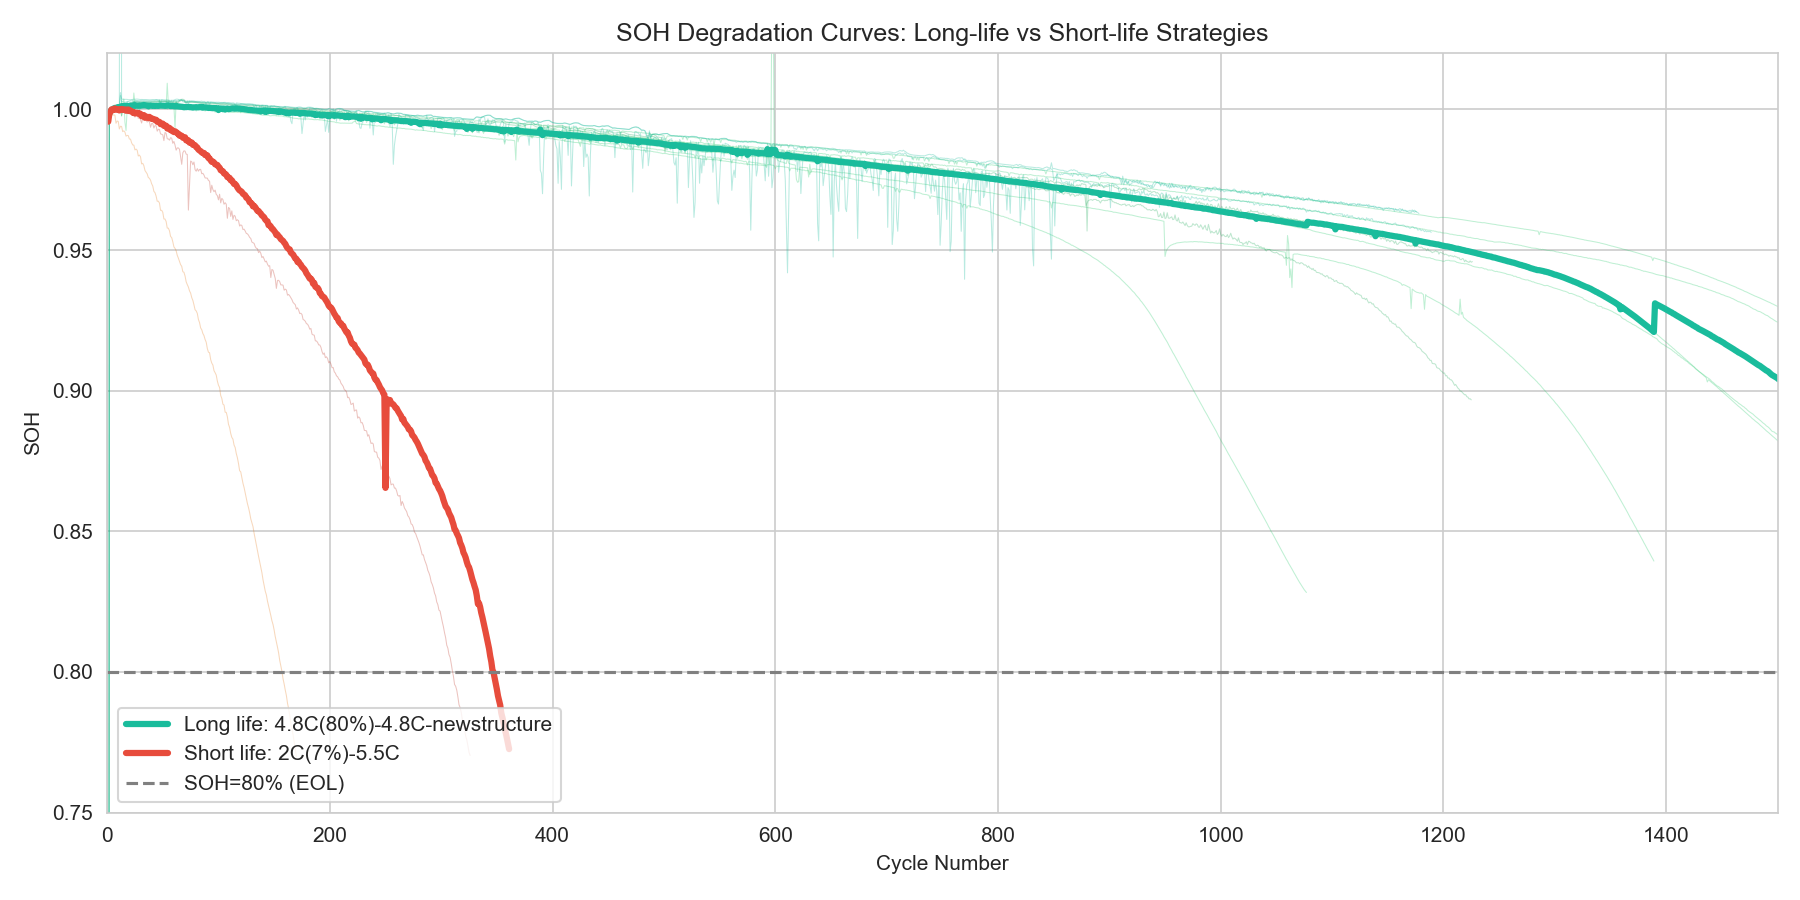
\includegraphics[width=0.92\textwidth]{fig2_soh_curves.png}
\caption{长寿命与短寿命策略的SOH衰减曲线对比（粗线为中位数曲线，细线为各电池曲线）}
\label{fig:soh}
\end{figure}

\subsection{关键影响因素分析}

为定量评估各充电参数对循环寿命的影响，计算了各因素之间的Pearson相关系数矩阵，如图\ref{fig:corr}所示。

\begin{figure}[H]
\centering
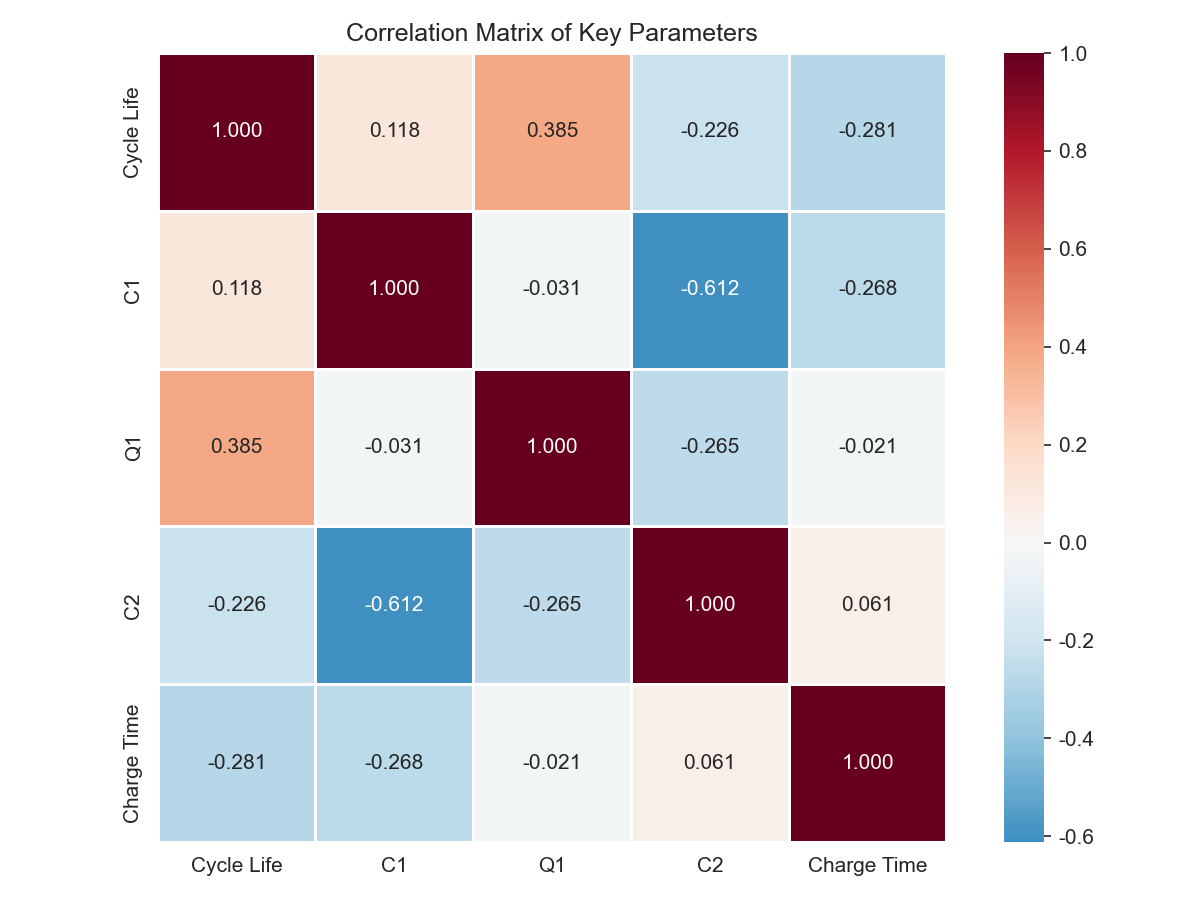
\includegraphics[width=0.65\textwidth]{fig6_correlation.png}
\caption{关键参数相关性热力图}
\label{fig:corr}
\end{figure}

基于相关性分析和散点图，得出以下核心发现：

\subsubsection{发现一：SOC切换节点$Q_1$是关键分水岭}

\begin{figure}[H]
\centering
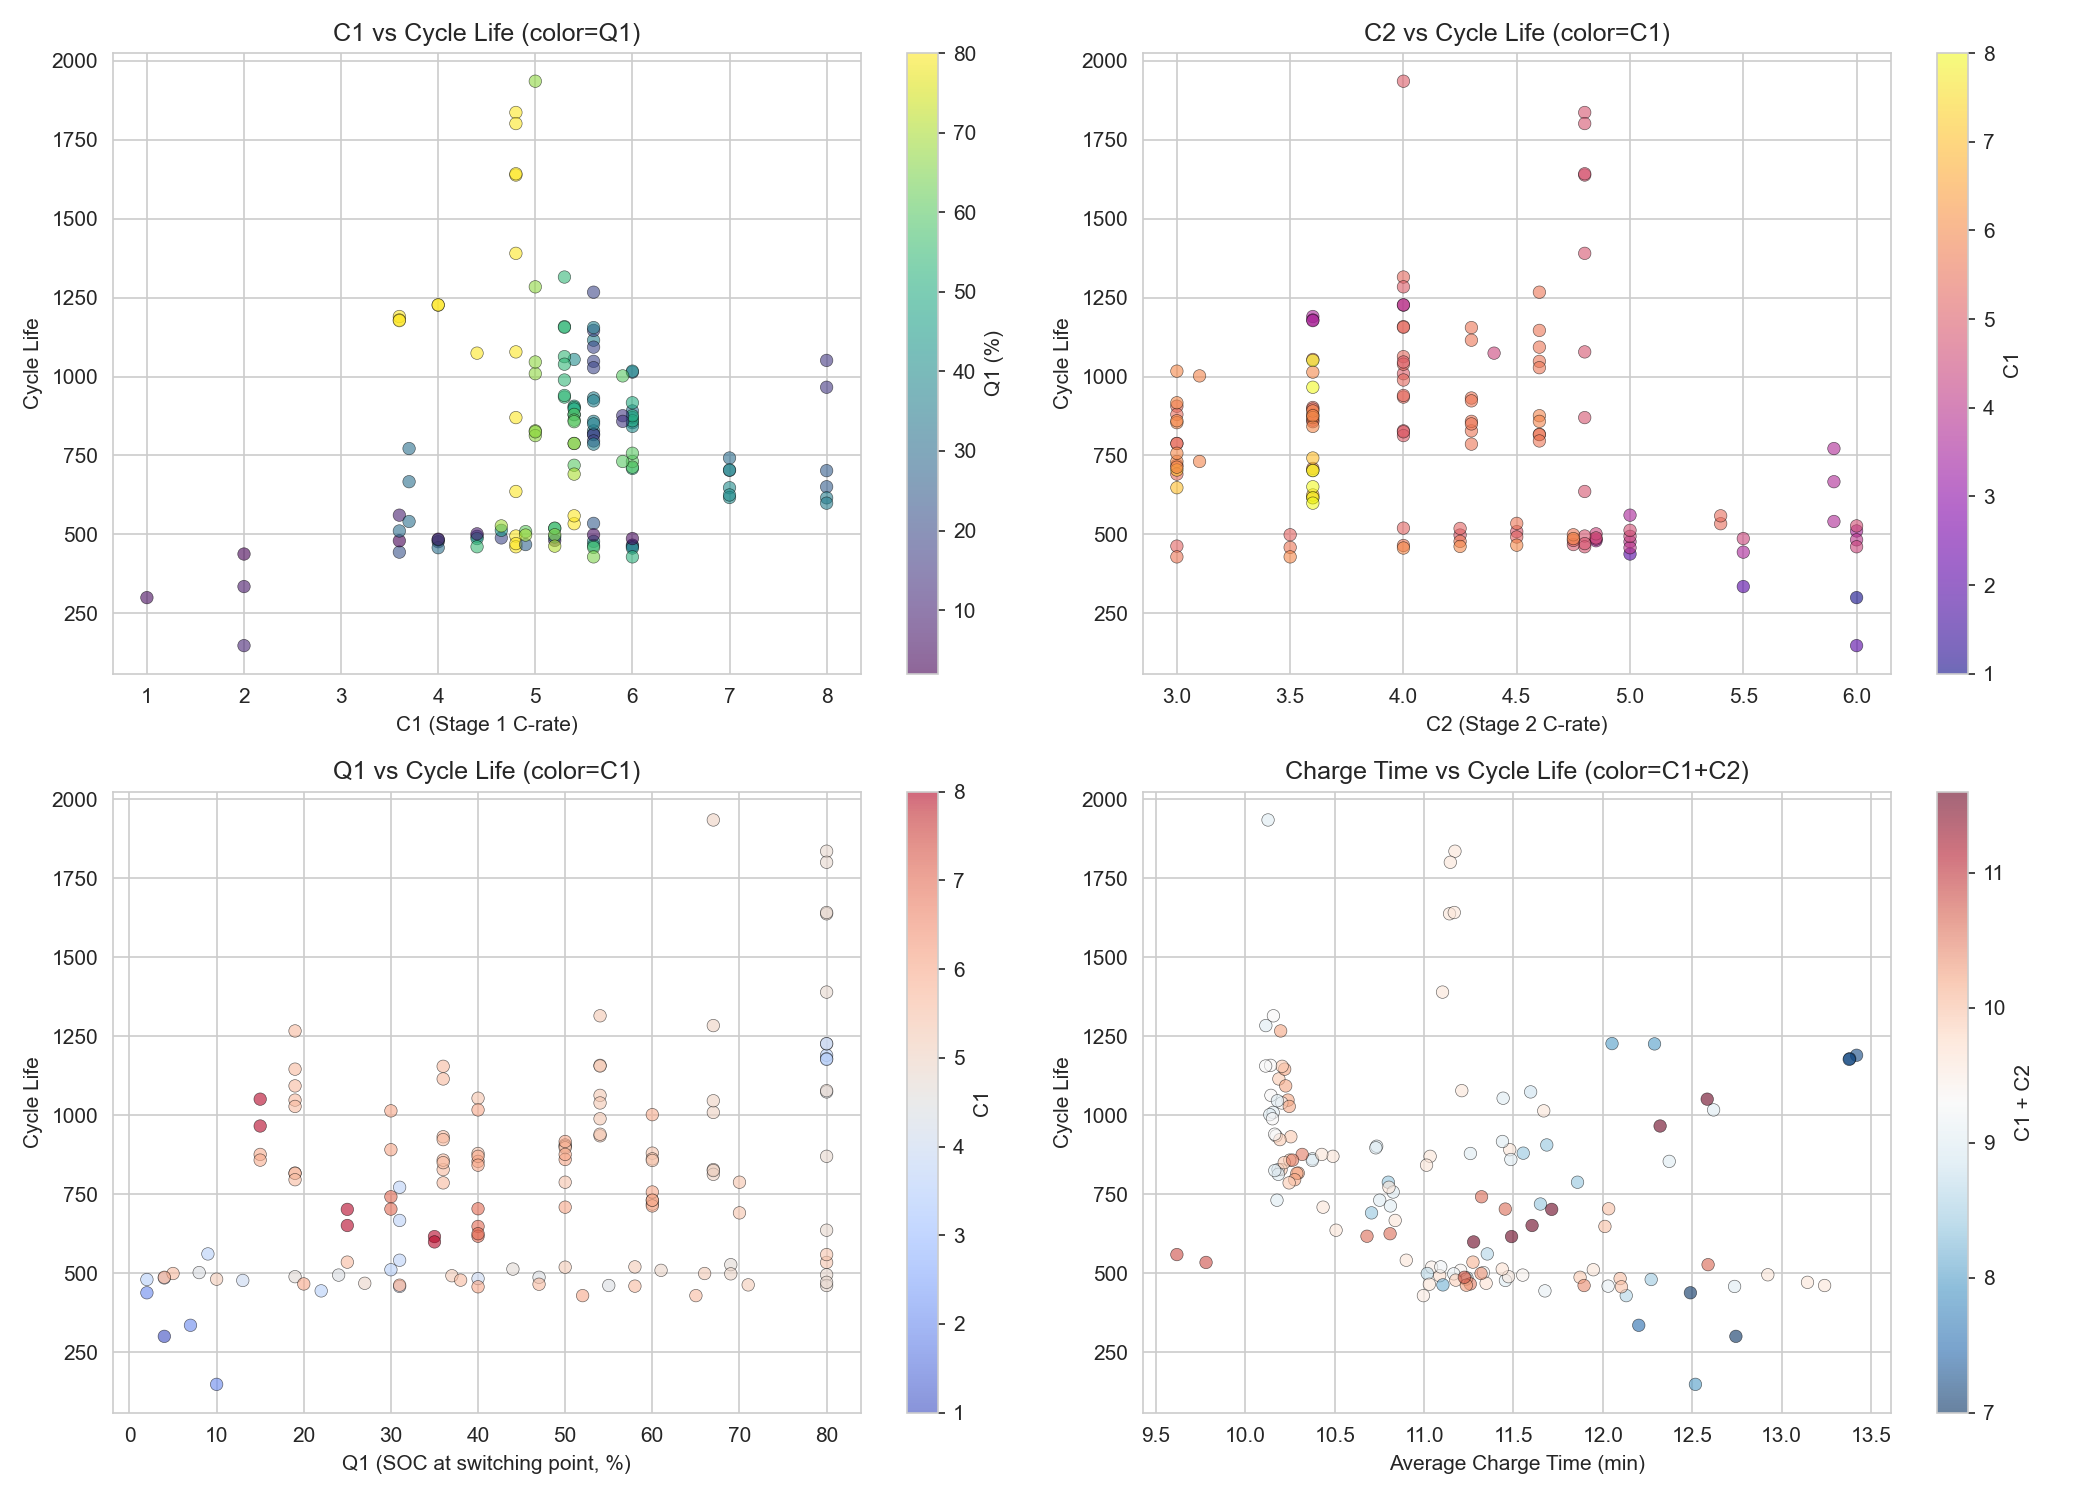
\includegraphics[width=0.65\textwidth]{fig3_param_vs_life.png}
\caption{充电策略参数与循环寿命的关系散点图}
\label{fig:scatter}
\end{figure}

长寿命策略的$Q_1$全部为80\%，即第一阶段覆盖整个0\%--80\% SOC区间。
这意味着充电电流在整个快充过程中保持均匀分配，避免了电流突变带来的极化冲击。
相反，短寿命策略的$Q_1$仅为4\%--10\%，第一阶段极短，第二阶段承担了绝大部分充电任务，
迫使电池在中高SOC区间承受过高倍率。

\subsubsection{发现二：第二阶段倍率$C_2$对寿命影响最大}

相关性分析显示，$C_2$与循环寿命呈显著负相关（$r \approx -0.56$）。
短寿命策略的$C_2$高达5.5C--6.0C，而长寿命策略的$C_2$仅为3.6C--4.8C。
这是因为$C_2$作用于中高SOC区间（$Q_1 \to 80\%$），该区间内电池极化增强、锂析出风险增大，
高倍率充电会显著加速副反应和容量衰减。

\subsubsection{发现三：低SOC区间对高倍率容忍度较高}

第一阶段倍率$C_1$与循环寿命的相关系数（$r \approx -0.27$）远小于$C_2$。
例如，策略``8C(35\%)-3.6C''的第一阶段采用8C超快充，但$C_2$仅为3.6C，寿命仍达到608次。
这说明低SOC区间（0\%--30\%左右）电池内阻较低，对高充电倍率的耐受性较强，
高倍率充电的损害主要集中在SOC较高的阶段。

\subsubsection{发现四：充电时间与寿命无简单线性关系}

从充电时间与循环寿命的散点图（图\ref{fig:scatter}右下）可以看出，
相近的充电时间下（约12分钟），寿命可从148次跨越至1227次，差异达8倍以上。
这表明单纯延长或缩短充电时间并不能直接决定电池寿命，关键在于充电电流在SOC区间上的分配方式。

\begin{figure}[H]
\centering
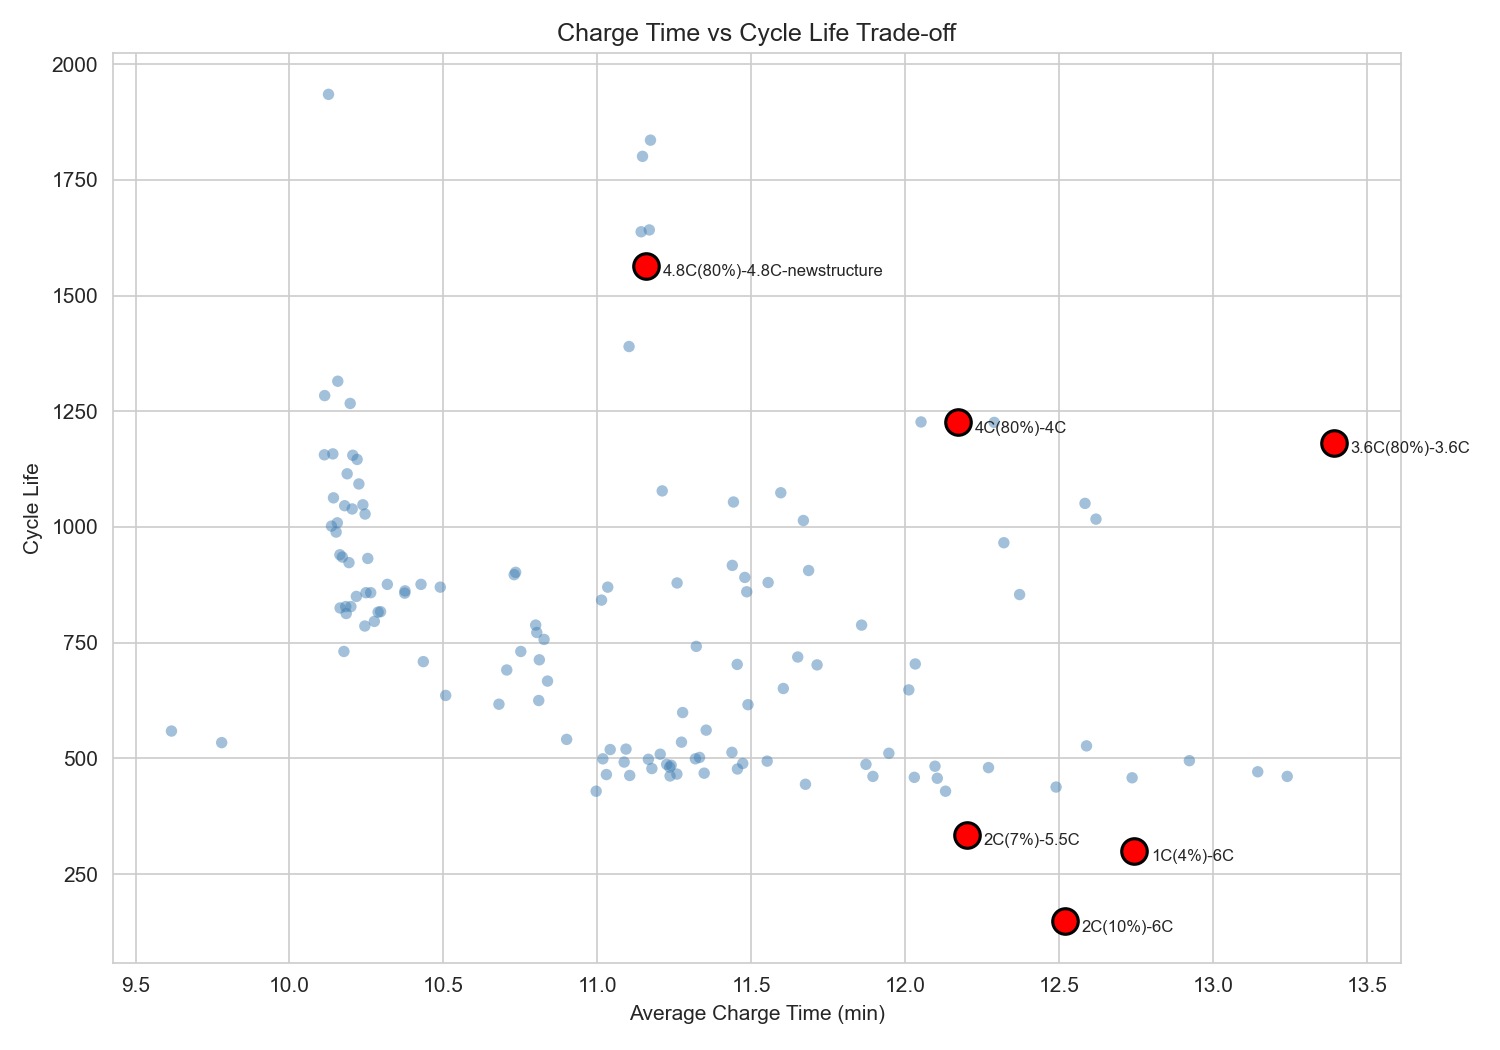
\includegraphics[width=0.65\textwidth]{fig5_tradeoff.png}
\caption{充电时间与循环寿命的权衡关系（红点为典型策略均值，已标注具体策略名称）}
\label{fig:tradeoff}
\end{figure}

\subsection{长寿命策略的共同特征}

归纳长寿命快充策略具备以下三个共同特征：
\begin{enumerate}
    \item $Q_1$较高（通常$\geq 80\%$），确保第一阶段覆盖大部分快充区间，避免SOC中途换挡带来的电流冲击；
    \item $C_2$与$C_1$的差异较小（$|C_1 - C_2| \leq 0.4$C），充电倍率在两阶段间平滑过渡；
    \item 总体倍率水平适中（$C_1, C_2 \in [3.6, 4.8]$），避免极端大电流带来的加速老化。
\end{enumerate}

\section{结论}

基于对133块电池、70种快充策略的系统分析，问题一得出以下主要结论：

\begin{enumerate}
    \item \textbf{充电策略对循环寿命影响极大}。最优策略（4.8C(80\%)-4.8C，平均1564次）的寿命是最差策略（2C(10\%)-6C，148次）的10倍以上。
    \item \textbf{SOC切换节点$Q_1$是区分长寿命与短寿命策略的核心参数}。$Q_1=80\%$的策略（第一阶段覆盖全部快充区间）表现最优，$Q_1 < 20\%$的策略几乎全部短寿。
    \item \textbf{第二阶段倍率$C_2$的影响大于第一阶段倍率$C_1$}。中高SOC区间的高倍率充电是加速老化的主要原因。
    \item \textbf{充电时间的绝对值不是决定寿命的关键}。相同充电时间下，通过合理分配SOC区间电流，可以显著延长电池循环寿命。
\end{enumerate}

这些发现为问题二的定量建模和问题四的策略优化提供了明确的建模方向和约束条件。

\begin{thebibliography}{9}
\bibitem{severson2019}
Severson K A, Attia P M, Jin N, et al.
Data-driven prediction of battery cycle life before capacity degradation[J].
\textit{Nature Energy}, 2019, 4(5): 383-391.
\end{thebibliography}

\end{document}
